\Chapter{Tervezés}

Ebben a fejezetben bemutatásra kerül a program koncepciója, céljai, tervezett működése. Feltérképezünk néhány nagyobb tervezési problémát és megkeressük a megoldásukat. Ennek céljából az OpenCL elemzendő részeinek további vizsgálata is megtörténik.

\Section{Koncepció}
Mint látni lehet a Multi2Sim-nél, a szimuláció lehetséges megoldása a problémának, viszont roppant bonyolult és erőforrásigényes. Ebben a dolgozatban megpróbálunk egy sokkal egyszerűbb, kevésbé pontos megoldást kínálni, ami remélhetőleg sokkal szemléletesebb. 

Mivel a hardveres futás szimuláció kicsit bonyolult, ezért azt elvetve marad a futó program elemzése. Erre lehetőséget biztosít a GDB \cite{gdb}, egy GNU project debugger, de ennek a precizitása kétséges, illetve csak a hoszt program futásának elemzésére alkalmas. A másik vizsgálandó megoldás a forráskód elemzése.

Az OpenCL működésének ismeretével lehetséges lehet olyan alkalmazást létrehozni, ami a forráskódban felismeri az OpenCL elemeit, és helyesen megtippeli, hogy azok mit csinálnának. Így felépíthető lenne egy modell az adott OpenCL program működéséről, amit már csak megjeleníteni szükséges.
 
\Section{Gazdaprogram elemei}
Az OpenCL programok egy jelentős része a hoszt programban történik, aminek nagyon sok kötelező eleme van, mint például a platformok keresése. Ezeket a program megkeresi és feljegyzi, hogy majd később megjeleníthesse őket. Legnagyobb részük 1 szálon szekvenciálisan fut, és OpenCL elemekkel dolgoznak, mint pédául DeviceID-kkal vagy OpenCL platformokkal. Elemzési teendő így nem nagyon van. Ekkor a hoszt program nagy része már modellezve is van.

Ilyen elem lehet a platform, memóriák felszabadítása, kernel létrehozás, OpenCL program készítése, parancssor készítése, környezet létrehozása, egyebek.



\Section{Teendők a kernellel}
Igazából a kernelben található konkrét műveletek elemzési, vizualizációs szempontokból elhanyagolhatók. Ami ott fontos, és ajánlott vele foglalkozni, azok a szinkronizációs függvények, például egy barrier-t érdemes lehet grafikusan megjeleníteni.

\Section{Munka elemek}
Egy fontosabb részlete az elemzésnek a munka elemek számának megállapítása. Ideális esetben meg van határozva a munkacsoport elemeinek száma, és ez kiolvasható a forráskódból. Ha ez nincs meghatározva, meg kell tippelnünk a számukat az OpenCL specifikáció alapján. Ezután rá tudunk jönni a munkacsoportok számára az \textit{NDRange} és a kernel input alapján.

\Section{Program feladatai}
Az alkalmazás feladatai tehát a következők:
\begin{itemize}
\item\textbf{Böngészős felhasználói felület:} Legyen az alkalmazásnak egy grafikus, interaktív felhasználói felülete. Ezt a felületet bármilyen böngészőn át képesek legyünk elérni.
\item\textbf{Fájl feltöltés:} A JavaScript nem teszi lehetőve a fájlok kliensoldali kezelését, ezért el kell őket juttatni a szerverhez. Biztonsági okokból a fájlok helyéhez sem fér hozzá a böngésző, így a tényleges fájlt kell feltölteni.
\item\textbf{Architektúra elemzése:} A szervernek képesnek kell lenni a szervert futtató számítógép hardverének a felismerésére, és abból következtetéseket levonni. Ha nincs mód a hardver információk gyűjtésére, akkor "kitalált" hardvert kell elemezni.
\item\textbf{OpenCL elemek vizsgálata:} A szervernek vizsgálni kell a forrásfájlban található OpenCL utasításokat, és grafikusan ábrázolni őket.
\item\textbf{Kernel szimuláció:} A szervernek képesnek kell a kernelt vizsgálni, szimulálni. A vizsgálat alapján információkat grafikusan megjeleníteni.
\end{itemize}


\Section{Program felépítése}



A program működése a következő lépésekben történik.

A webalkalmazáson át feltöltünk egy forrásfájlt, majd a szerver a fájlt beolvassa soronként. Megvizsgálja, hogy a forrásfájl milyen OpenCL eszközöket használ, hány munka elem van benne, stb. A szerver ezután lekéri a számítógép architektúráját. Következő lépésben a webalkalmazás megrajzolja a számítógép ide vonatkozó Hardware elemeit, mint a rendelkezésre álló memória, a processzor adatai, a videókártya adatai, valamint felvázolja, hogy az architektúrát milyen módon használná az OpenCL program. A szerver megkeresi a forrásfájlban az OpenCL függvényeket, és szükségszerűen modelleket rendel hozzájuk, vagyis megfelelő objektumokat hoz létre. Például a \texttt{clCreateKernel} metódust észlelve létrehozunk egy Kernel objektumot. Ilyenkor azt is megállapítja, hogy az adott elem melyik számítási egységhez tartozik. Ha ez sikeres, a webalkalmazás egy Gantt diagramban vizualizálja a program futtatását az idő függvényében. A webalkalmazás ezzel szinkronban megjeleníti magát a forráskódot is, és bármely Gantt diagrambeli elemre kattintva kiemeli a megfelelő kódot. A program ezen részének UML diagramja \aref{fig:uml} ábrán látható. Az ábrából hiányoznak típusok és paraméterek, mert ebben a fázisban még nem tudni, hogy mik lesznek.

\begin{figure}[h!]
\centering
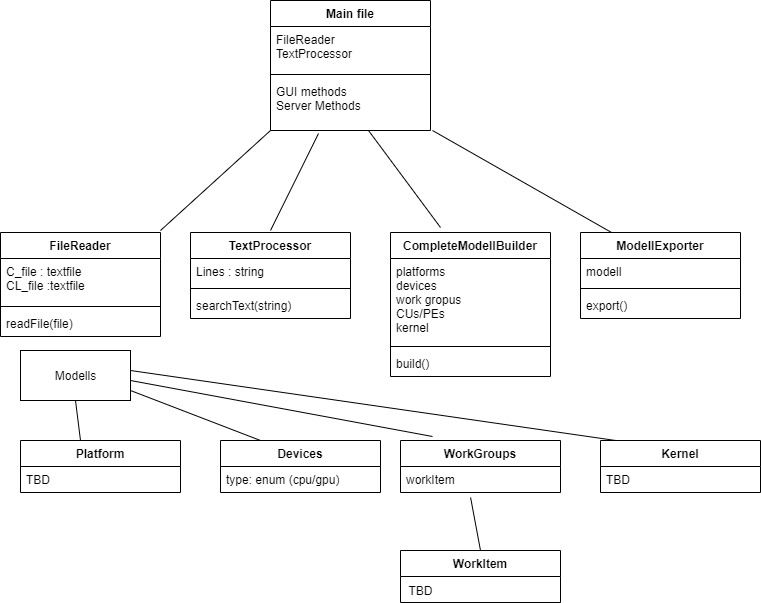
\includegraphics[width=\textwidth]{images/UML.jpg}
\caption{Részleges UML osztálydiagram}
\label{fig:uml}
\end{figure}

A program másik fele az Aritmetikai szimulációval foglalkozik. Ennek szükséglete lenne a forrásfájl "lefordítása" és futtatása, viszont a fordítás teljes folyamatának bemutatása, elemzése nem célja a dolgozatnak.

\begin{figure}[h!]
\centering
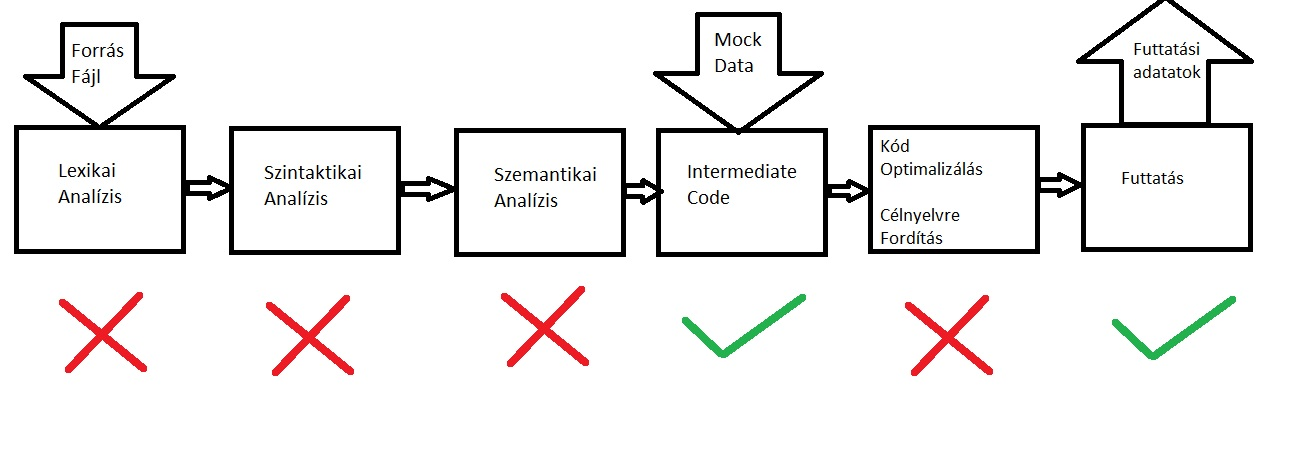
\includegraphics[width=\textwidth]{images/Compiler.jpg}
\caption{Fordító és módosításai}
\label{fig:compiler}
\end{figure}

Egyik lehetőség az elemzésre a parzolás volt, amire az ANTLR parser generátorral generált parzer tűnt alkalmasnak \cite{antlr}, mert elérhető hozzá nagyon sok nyelvtan, többek között C nyelvtan is. Az ANTLR nemrég bővítette célnyelveit C{\#}-al, tehát ebből a szempontból is megfelelő lett volna. Az ANTLR az adott nyelvtannak megfelelően generál Token-eket, Lexer-t és Parser-t. Ezután egy input-ra fel tudunk építeni egy parse fát, ha meg tudjuk mondani, hogy az input milyen nyelvtani elem. Ezután a fát tudjuk böngészni saját Listener-el vagy Visitor-al, és adatokat kinyerni belőle. Ez az irány akkor ért zsákutcába, amikor kiderült, hogy nem létezik olyan nyelvtani elem hogy “teljes C fájl”, és így nem lehet egy forrásfájlból parse fát létrehozni. Ha mégis e mellett döntöttem volna, akkor szükséges lett volna saját nyelvtan létrehozása.

Kompromisszumos megoldás az első lépések, vagyis a lexikai analízis, szintaktikai analízis, szemantikai analízis, illetve később a kód optimalizálás kihagyása (\ref{fig:compiler} ábra). A szimuláció így "kitalált" elemekkel dolgozik, amit vagy a fájlnév alapján hoz létre, vagy mi magunk adhatunk meg. Ezek az elemek az intermediate code, azaz átmeneti kód elemei, amiket instrukcióknak nevezünk. Ha ezek megvannak, akkor az alkalmazás szimulálja őket, feljegyzi a instrukció lépés számot, a minimális memória igényt, és a futási időt, valamint létrehoz egy szintaktikai fát az instrukciók alapján. A szimuláció ténylegesen elvégzi a lépéseket, létrehoz változókat, műveleteket végez rajtuk, és végül kiírja az eredményeket. A szimulációhoz tartozó UML diagram \aref{fig:simUML} ábrán látható.

\begin{figure}[h]
\centering
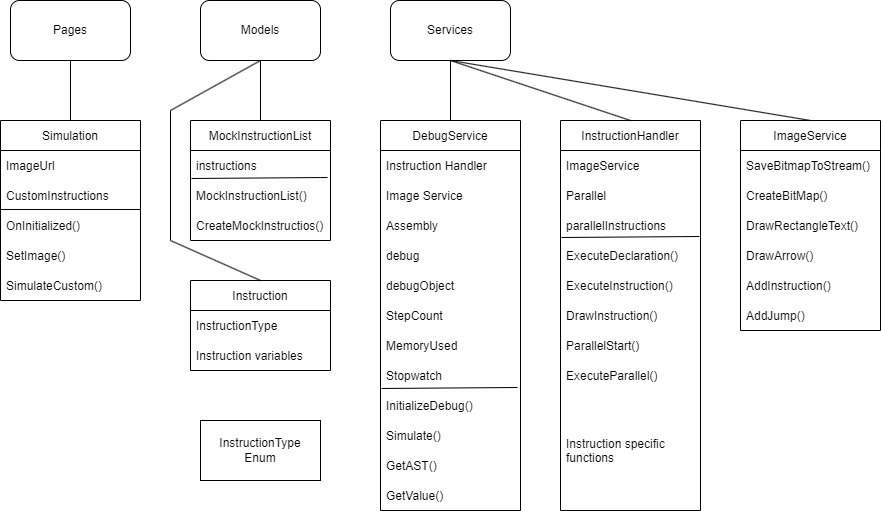
\includegraphics[width=\textwidth]{images/SimUML.jpg}
\caption{Szimulációs részlet UML diagramja}
\label{fig:simUML}
\end{figure}






%\Section{Táblázatok}

%Táblázatokhoz a \texttt{table} környezetet ajánlott használni.
%Erre egy minta \aref{tab:minta}. táblázat.
%A hivatkozáshoz az egyedi \texttt{label} értéke konvenció szerint \texttt{tab:} prefixszel kezdődik.

%\begin{table}[h]
%\centering
%\caption{Minta táblázat. A táblázat felirata a táblázat felett kell legyen!}
%\label{tab:minta}
%\begin{tabular}{l|c|c|}
%a & b & c \\
%\hline
%1 & 2 & 3 \\
%4 & 5 & 6 \\
%\hline
%\end{tabular}
%\end{table}

%\Section{Ábrák}

%Ábrákat a \texttt{figure} környezettel lehet használni.
%A használatára egy példa \aref{fig:cimer}. ábrán látható.
%Az \texttt{includegraphics} parancsba 
%Az ábrák felirata az ábra alatt kell legyen.
%Az ábrák hivatkozásához használt nevet konvenció szerint \texttt{fig:}-el célszerű kezdeni.

%\begin{figure}[h]
%\centering
%
\includegraphics[scale=0.3]{images/me_logo.png}
%\caption{A Miskolci Egyetem címere.}
%\label{fig:cimer}
%\end{figure}

%\Section{További környezetek}

%A matematikai témájú dolgozatokban szükség lehet tételek és bizonyításaik megadására.
%Ehhez szintén vannak készen elérhető környezetek.

%\begin{definition}
%Ez egy definíció
%\end{definition}

%\begin{lemma}
%Ez egy lemma
%\end{lemma}

%\begin{theorem}
%Ez egy tétel
%\end{theorem}

%\begin{proof}
%Ez egy bizonyítás
%\end{proof}

%\begin{corollary}
%Ez egy tétel
%\end{corollary}

%\begin{remark}
%Ez egy megjegyzés
%\end{remark}

%\begin{example}
%Ez egy példa
%\end{example}
